
Based on the courses discussed above, we measured each algorithm's ability to solve tests based on a selected timeout against the wall clock time (in $\log(s)$). This helps us analyze how many and how fast each algorithm can solve tests within the 5-minute timeout per test for $d>2$ solvers and 1-second timeout per test for $d=2$ solvers in each course. Moreover, measuring wall clock time in $\log(s)$ helps visualize data more effectively as the data points are distributed more evenly.  \\
These performance graphs are designed to provide an intuitive comparison of the algorithms. The closer each algorithm's performance line is to the y-axis, the faster the algorithm completes its tests, indicating a lower wall clock time. Additionally, the higher a line is on the graph, the more tests the algorithm successfully solved, showing its accuracy, and effectiveness. To evaluate overall performance, we consider both these aspects. A fast algorithm that can only solve a few tests could indicate that the algorithm got "lucky" with certain test cases. An accurate algorithm that is slow could suggest that it produces relatively better results while compromising speed.


\subsubsection*{Course 1: Perfect Matching}

\begin{figure}[h!]
    \centering
    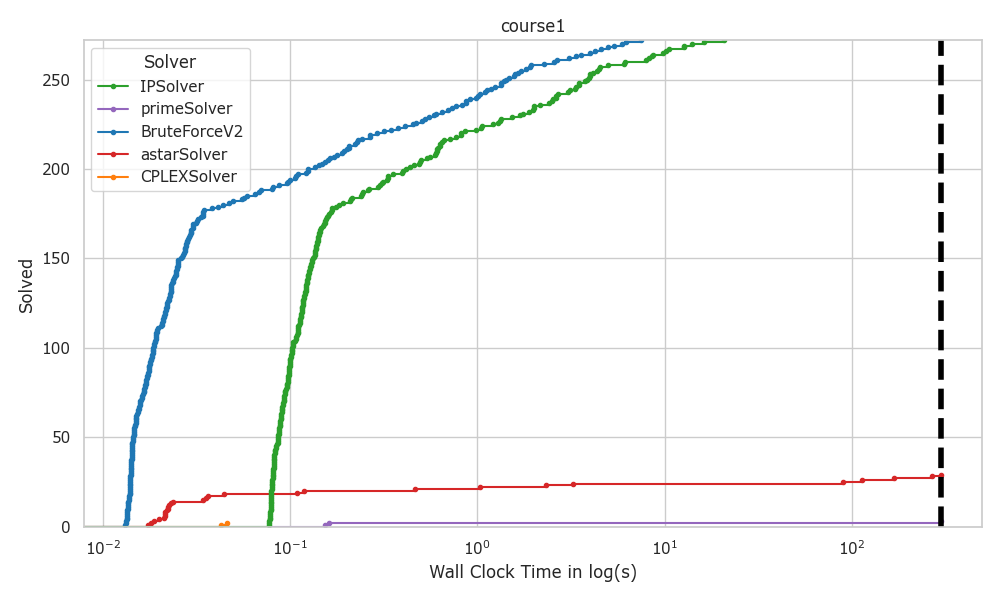
\includegraphics[width=\textwidth]{Graphs/course1.png}
    \caption{Performance of solvers on course 1}
\end{figure}

For course 1, the graph demonstrates clear differences in the performance of the solvers. The \textbf{BruteForceV2} solver, represented in blue, is both the fastest and the most accurate, solving all the tests within a shorter wall clock time. The \textbf{IPSolver}, shown in green, also solves a high number of tests, but it is slightly slower compared to BruteForceV2. Other solvers, such as \textbf{CPLEXSolver} (orange) and \textbf{primeSolver} (purple), perform very poorly as they were only able to solve a small fraction of the tests, and they were also not very fast on the tests they passed. The \textbf{astarSolver} (red) was able to solve more tests than CPLEXSolver and primeSolver but failed to compete with BruteForceV2 or IPSolver in both speed and accuracy. Overall, for a perfect matching scenario, BruteForceV2 demonstrates the best performance, followed closely by IPSolver, while the remaining solvers show limited efficiency in this course.

\subsubsection*{Course 2: Random Matching (non-perfect)}

\begin{figure}[h!]
    \centering
    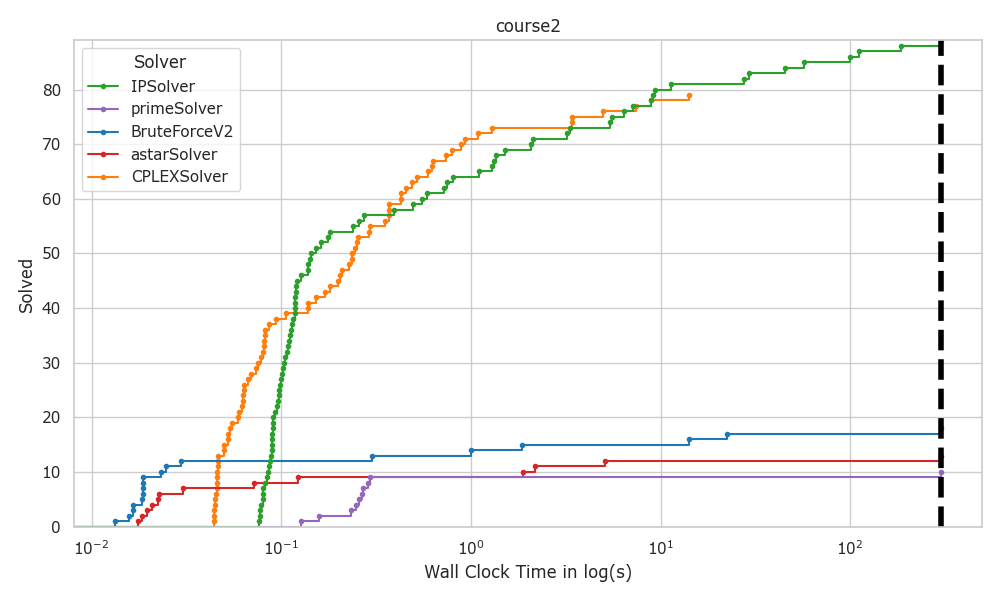
\includegraphics[width=\textwidth]{Graphs/course2.png}
    \caption{Performance of solvers on course 2}
\end{figure}

For course 2, the \textbf{IPSolver} (green) outperforms the others, solving the highest number of tests while also maintaining a relatively high speed. The \textbf{CPLEXSolver} (orange) also performs well, solving nearly as many tests as IPSolver, though it is slightly slower on some tests. The \textbf{BruteForceV2} (blue), while both accurate and fast on course 1, struggles in a non-perfect matching scenario, solving far fewer tests and taking considerably more time. Similarly, the \textbf{astarSolver} (red) and \textbf{primeSolver} (purple) also show limited performance, solving only a small fraction of tests with significantly slower speeds. Overall, for a non-perfect scenario, the IPSolver outperforms the other solvers, both in efficiency and effectiveness for course 2, with CPLEXSolver having a very similar performance.

\subsubsection*{Course 3: $\vert$Max-Matching$\vert$ in $[n/2,3n/4)$}

\begin{figure}[h!]
    \centering
    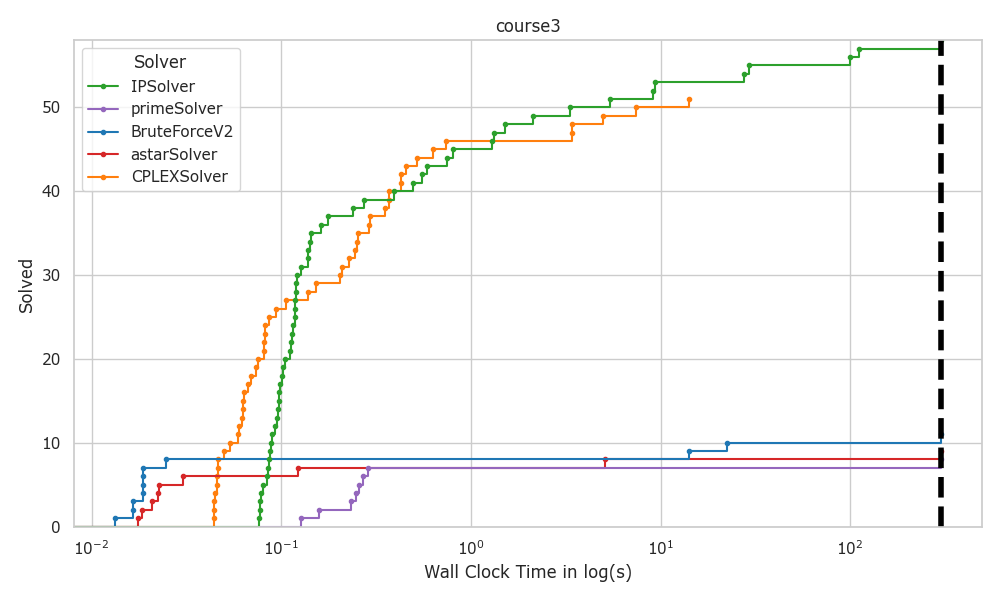
\includegraphics[width=\textwidth]{Graphs/course3.png}
    \caption{Performance of solvers on course 3}
\end{figure}

For course 3, the \textbf{IPSolver} (green) again performs better than other solvers, solving the highest number of tests while maintaining a low wall clock time. The \textbf{CPLEXSolver} (orange) closely follows IPSolver, solving a comparable number of tests at a similar speed. Thus, both solvers demonstrate strong accuracy and efficiency. Other solvers including \textbf{BruteForceV2} (blue), \textbf{astarSolver} (red) and \textbf{primeSolver} (purple) perform poorly, solving only a small number of tests with longer computation times. Overall, IPSolver and CPLEXSolver significantly outperform other solvers in both speed and effectiveness for course 3 where the size of matching lies in the fourth quartile.

\subsubsection*{Course 5: Large $n$ $(>1000)$}
\begin{figure}[h!]
    \centering
    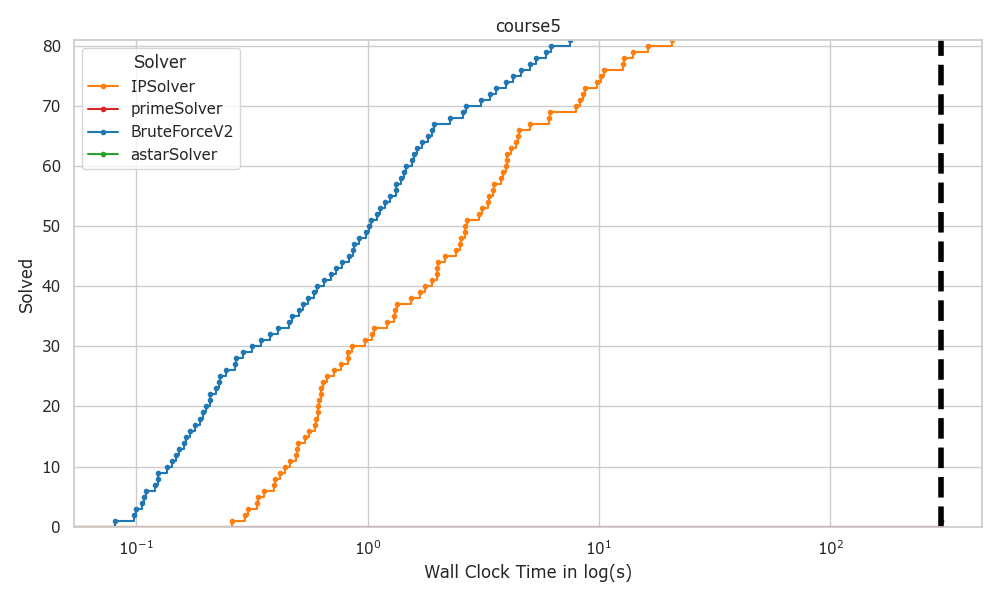
\includegraphics[width=\textwidth]{Graphs/course5.png}
    \caption{Performance of solvers on course 5}
\end{figure}

For course 5, we were only able to gather data for \textbf{BruteForceV2} (blue) and \textbf{IPSolver} (orange). Other solvers were not able to run any tests for large amounts of vertices within the 5-minute timeout. The BruteForceV2 solver performs slightly better compared to the IPSolver, however, their performances are very similar. Both were able to solve around 80 test cases within the timeout. However, this result is not fully reflective of the provided criteria as most of the tests that were generated had a perfect matching.  Overall, BruteForceV2 and IPSolver significantly outperform other solvers for course 5 where the graphs have a large size.

\subsubsection*{Course 8: Small $m$ ($< \frac{n^d}{2}$) - Sparse Graphs}

\begin{figure}[h!]
    \centering
    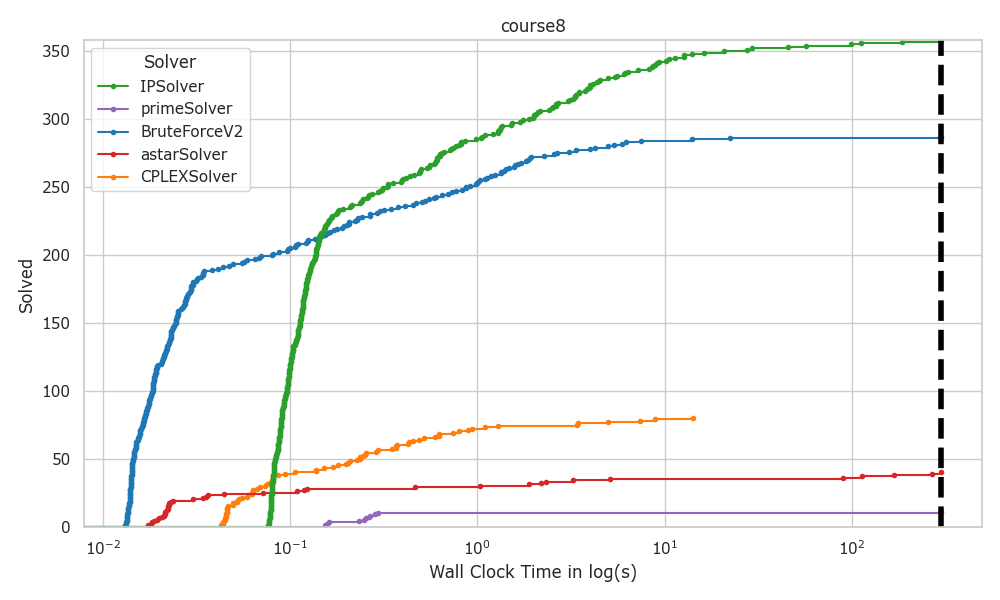
\includegraphics[width=\textwidth]{Graphs/course8.png}
    \caption{Performance of solvers on course 8}
\end{figure}

For course 8, the \textbf{IPSolver} (green) was able to solve the highest number of tests while maintaining a relatively low wall clock time. However, the \textbf{BruteForceV2} (blue) was able to solve around 200 test cases faster than the other solvers. Thus, both solvers demonstrate strong performance in this course. Other solvers including \textbf{astarSolver} (red), \textbf{CPLEXSolver} (orange) and \textbf{primeSolver} (purple) perform poorly in this course, solving only a small number of tests. Overall, IPSolver is more accurate than other solvers while the BruteForceV2 solver is faster for course 8 where the graphs are sparse and have a low number of edges.

\subsubsection*{Course 9: Easy problems with small $n$ $(<100)$ and $m$ $(<50)$ values}

\begin{figure}[h!]
    \centering
    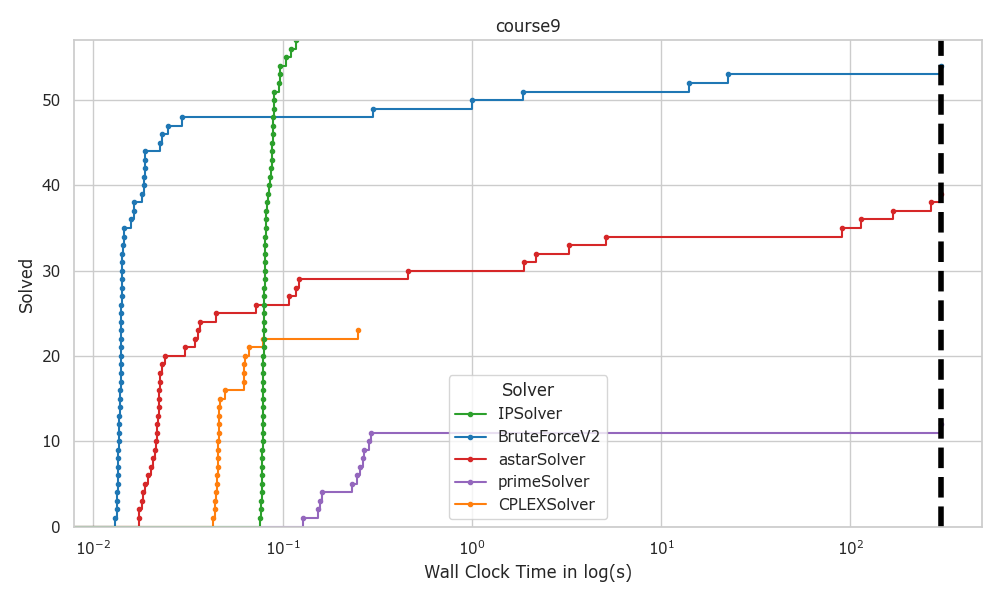
\includegraphics[width=\textwidth]{Graphs/course9.png}
    \caption{Performance of solvers on course 9}
\end{figure}

For course 9, the \textbf{BruteForceV2} (blue) and \textbf{IPSolver} (green) were able to solve the highest number of tests. However, due to the lack of test data, these graphs may not accurately reflect the true performance of the algorithms. Thus, more data would have given a more conclusive result for this course. Based on the results, the BruteForceV2 solver was the fastest with relatively higher accuracy while the IPSolver was the most accurate. Other solvers also performed well but failed to solve most of the test cases.


\subsubsection*{Overall Results}

Dividing Races into different courses allowed us to see how each algorithm behaves in different scenarios of the problem. Across all courses, the IPSolver consistently demonstrates strong performance, solving the highest number of tests in most scenarios while maintaining relatively low wall clock times. Moreover, it outperformed most of the other solvers in random matching (Course 2), larger size Max-Matching (Course 3,) and sparse graph scenarios (Course 8). Similarly, the BruteForceV2 solver demonstrates better performance on more structured problems like perfect matching (Course 1), large graphs (course 5), and easier problems (Course 9). However, it struggled with larger or more complex graph scenarios, like Course 2 and Course 3. The CPLEXSolver shows competitive performance in specific scenarios like random matching (Course 2) and large-sized matching (Course 3) but underperforms in other courses. Meanwhile, both the astarSolver and primeSolver are less competitive, solving significantly fewer tests across all courses and being slower compared to other solvers.


\subsubsection*{Limitations and Future Work}

One of the main limitations of this study is the inability to generate sufficient data, specifically for Courses 4, 6, and 7. Due to the complexity of generating test cases for these courses, we were unable to produce meaningful visualizations or comparisons for these scenarios. 

Another limitation lies in the relatively small number of test cases generated for some of the courses. A larger number of test cases, along with an increased timeout duration for computational experiments, would provide a better evaluation of solver performance, particularly for large graphs or highly complex scenarios. Additionally, the solvers might demonstrate different performances if tested over a broader range of problems and parameters.

In the future, we focus on refining the design of the courses by looking at multiple parameters to capture more details of solver performance. Moreover, having proper development tools to generate tests based on a specification will greatly benefit testing with a broader range of values. Overall, with more test data, improved parameter tuning, and enhanced tools for generating challenging scenarios, we can provide a deeper understanding of solver performance across diverse scenarios.
